% ============================================================
% Capítulo I — Estudio de los pequeños movimientos en un medio elástico
% Traducción de "Théorie mathématique de la lumière" (1889), cap. I
% Original: §§1-39, páginas 3-48
% ============================================================
\chapter{Estudio de los pequeños movimientos en un medio elástico}
\label{cap:movimientos-pequenos}

\noindent\textbf{1. Primera hipótesis.} — Consideraremos un medio elástico
formado por moléculas separadas unas de otras; es decir, admitiremos la
discontinuidad de la materia. Observemos que la concordancia de los hechos
experimentales con las consecuencias matemáticas obtenidas a partir de esta
hipótesis no es una prueba de la discontinuidad de la materia. Esta
hipótesis solo tiene por efecto simplificar los cálculos; podría suponerse
la materia continua y la concordancia que señalamos subsistiría de todos
modos.

\begin{enunciado}{Primera hipótesis}
El medio elástico está formado por moléculas separadas unas de otras: se
admite la discontinuidad de la materia.
\end{enunciado}

\noindent\textbf{2. Segunda hipótesis.} — Admitiremos que las moléculas
están sometidas a ciertas fuerzas, que existe una posición de equilibrio
estable del medio, y que, si se separan las moléculas de sus posiciones de
equilibrio y luego se abandonan a sí mismas, toman movimientos de
oscilación muy pequeños alrededor de su posición de equilibrio.

\begin{enunciado}{Segunda hipótesis}
Las moléculas están sometidas a ciertas fuerzas; existe una posición de
equilibrio estable del medio, y si se separan las moléculas de esa
posición y luego se abandonan a sí mismas, toman movimientos de oscilación
muy pequeños alrededor de ella.
\end{enunciado}

\section{Ecuaciones del movimiento. La función de fuerzas}

\noindent\textbf{3. Ecuaciones del movimiento.} — Consideremos $n$
moléculas $\mathrm{M}_1,\mathrm{M}_2,\ldots,\mathrm{M}_i,\ldots$ de masas
$m_1,m_2,\ldots,m_i,\ldots$. Las coordenadas de una de estas moléculas serán,
en la posición de equilibrio, $x_i,y_i,z_i$; después del desplazamiento,
$x_i+\xi_i,\,y_i+\eta_i,\,z_i+\zeta_i$. Admitiremos que existe una función de
fuerzas $\mathrm{U}$, es decir, que hay conservación de la energía. Las
ecuaciones del movimiento de la molécula $\mathrm{M}_i$ serán:
\begin{equation}
m_i\frac{d^2\xi_i}{dt^2}=\frac{d\mathrm{U}}{d\xi_i},\qquad
m_i\frac{d^2\eta_i}{dt^2}=\frac{d\mathrm{U}}{d\eta_i},\qquad
m_i\frac{d^2\zeta_i}{dt^2}=\frac{d\mathrm{U}}{d\zeta_i}.
\tag{1}
\end{equation}

\noindent\textbf{4. Propiedades de la función de fuerzas.} — Si se desarrolla
$\mathrm{U}$ según las potencias crecientes de las $\xi$ (designando por
$\xi$ el conjunto de las cantidades $\xi_1,\eta_1,\zeta_1;\xi_2,\eta_2,\zeta_2,\ldots$),
se tiene:
\[
\mathrm{U}=\mathrm{U}_0+\mathrm{U}_1+\mathrm{U}_2+\mathrm{U}_3\ldots
\]
$\mathrm{U}_0$, que representa el término constante, puede suponerse nulo,
pues la función $\mathrm{U}$ solo interviene en las ecuaciones del
movimiento a través de sus derivadas.

$\mathrm{U}_1$, que representa el conjunto de los términos de primer grado
respecto de las $\xi$, es decir
\[
\sum \xi_i\left(\frac{d\mathrm{U}}{d\xi_i}\right)_0
\]
es nulo, pues $\dfrac{d\mathrm{U}}{d\xi_i}$ representa la proyección sobre
$\mathrm{O}x$ de la fuerza que se ejerce sobre la molécula $\mathrm{M}_i$,
fuerza que es nula en la posición de equilibrio, es decir, para $\xi_i=0$;
$\left(\dfrac{d\mathrm{U}}{d\xi_i}\right)_0$ es nulo, y por tanto
$\mathrm{U}_1$ también.

Finalmente, como las cantidades $\xi$ se suponen muy pequeñas (§2), se pueden
despreciar los términos de grado superior al segundo respecto de las $\xi$,
y se tiene simplemente:
\begin{equation}
\mathrm{U}=\mathrm{U}_2.
\tag{2}
\end{equation}

$\mathrm{U}_2$ es una forma cuadrática respecto de las $3n$ cantidades
$\xi$; se puede, pues, ponerla en forma de suma de cuadrados. Esta suma debe
ser negativa, pues, siendo estable el equilibrio cuando las $\xi$ son
nulas, la función $\mathrm{U}$ debe pasar por un máximo para $\xi=0$, y una
de las condiciones para que una función pase por un máximo es que el
conjunto de los términos de segundo grado del desarrollo sea negativo.

Si se dividen las fuerzas que actúan sobre el sistema en dos grupos,
fuerzas interiores y fuerzas exteriores, y se designa por $\mathrm{U}'$ la
función de fuerzas relativa al primer grupo, por $\mathrm{U}''$ la relativa
al segundo grupo, tendremos:
\begin{equation}
\mathrm{U}=\mathrm{U}'+\mathrm{U}''.
\tag{3}
\end{equation}

\noindent\textbf{5. Propiedades de las funciones $\mathrm{U}'$ y
$\mathrm{U}''$.} — Si las distintas moléculas se desplazan de manera que
sus distancias respectivas no varíen, el trabajo de las fuerzas interiores
es nulo; $\mathrm{U}'$ es entonces nula. $\mathrm{U}'$ puede, pues,
considerarse como una función de la distancia de las moléculas. Designando
por $\mathrm{R},\mathrm{R}',\ldots$ los cuadrados de estas distancias,
pondremos:
\begin{equation}
\mathrm{U}'=\mathrm{F}(\mathrm{R},\mathrm{R}',\mathrm{R}'',\ldots).
\tag{4}
\end{equation}

\noindent\textbf{6.} Si suponemos que dos moléculas $\mu$ y $\mu'$ se
atraen o se repelen según fuerzas iguales, dirigidas según la recta que las
une, y que no dependen más que de la distancia $\mu\mu'$ —en otros
términos, si nos situamos en la hipótesis de las fuerzas centrales—,
$\mathrm{U}'$ será la suma de las funciones de fuerzas relativas a dos
moléculas $\mu$ y $\mu'$; tendremos en este caso:
\begin{equation}
\mathrm{U}'=f(\mathrm{R})+f'(\mathrm{R}')+f''(\mathrm{R}'')+\ldots
\tag{5}
\end{equation}

\noindent\textbf{7.} Las fuerzas exteriores al sistema pueden ser de dos
especies: 1.\textsuperscript{o} las fuerzas que se ejercen a la vez sobre
las moléculas interiores y sobre las moléculas superficiales, como, por
ejemplo, las fuerzas debidas a la gravedad; 2.\textsuperscript{o} las
fuerzas que solo actúan sobre las moléculas superficiales, como las que se
ejercen sobre la superficie interna de las paredes de un recinto que
contiene un gas.

Las fuerzas del primer grupo no se presentan en óptica, pues se supone que
el éter es imponderable. En cuanto a las del segundo grupo, no tenemos
derecho a negar su existencia. Si suponemos que no existen, la función de
fuerzas relativa a las fuerzas exteriores al sistema es nula. Se tiene
entonces $\mathrm{U}''=0$.

\noindent\textbf{8.} Podemos desarrollar las funciones $\mathrm{U}'$ y
$\mathrm{U}''$ según las potencias crecientes de las $\xi$, y tendremos,
despreciando las potencias de las $\xi$ superiores al segundo grado:
\[
\mathrm{U}'=\mathrm{U}'_0+\mathrm{U}'_1+\mathrm{U}'_2,\qquad
\mathrm{U}''=\mathrm{U}''_0+\mathrm{U}''_1+\mathrm{U}''_2.
\]
Identificando el desarrollo de la función $\mathrm{U}$ (§4) con la suma de
las funciones $\mathrm{U}'$ y $\mathrm{U}''$ desarrolladas, obtendremos las
relaciones siguientes:\footnote{El original impreso dice
$\mathrm{U}'_1+\mathrm{U}''_2$ en el primer miembro de (7); es una errata
evidente por $\mathrm{U}'_2+\mathrm{U}''_2$, como confirma el uso que se hace
de (7) en los §§11 y 13.}
\[
\mathrm{U}'_0+\mathrm{U}''_0=\mathrm{U}_0=0.
\]
\begin{align}
\mathrm{U}'_1+\mathrm{U}''_1&=\mathrm{U}_1=0.\tag{6}\\
\mathrm{U}'_2+\mathrm{U}''_2&=\mathrm{U}_2=\mathrm{U}.\tag{7}
\end{align}
Podemos, por lo demás, suponer que las constantes $\mathrm{U}'_0$ y
$\mathrm{U}''_0$ son separadamente nulas.

\section{Estudio de la función $\mathrm{U}'$}

\noindent\textbf{9.} Sean dos moléculas $\mu$ y $\mu'$, cuyas coordenadas
están, en la posición de equilibrio,
\[
x,y,z,\qquad x+\mathrm{D}x,\;y+\mathrm{D}y,\;z+\mathrm{D}z,
\]
Designamos con la notación $\mathrm{D}x$ el incremento de una de las
coordenadas, pues la distancia de estas moléculas vecinas no es
infinitamente pequeña. El cuadrado de esta distancia es:
\[
\mathrm{R}=\mathrm{D}x^2+\mathrm{D}y^2+\mathrm{D}z^2.
\]
Si se separan estas moléculas de sus posiciones de equilibrio, sus
coordenadas se convierten en:
\[
x+\xi,\;y+\eta,\;z+\zeta;\qquad
x+\mathrm{D}x+\xi+\mathrm{D}\xi,\;y+\mathrm{D}y+\eta+\mathrm{D}\eta,\;
z+\mathrm{D}z+\zeta+\mathrm{D}\zeta;
\]
y el cuadrado de su distancia es entonces:
\[
\mathrm{R}+\rho=\sum(\mathrm{D}x+\mathrm{D}\xi)^2
=\sum \mathrm{D}x^2+2\sum \mathrm{D}x\,\mathrm{D}\xi+\sum \mathrm{D}\xi^2.
\]
El incremento $\rho$ del cuadrado de esta distancia viene dado por la
relación:
\[
\rho=2\sum \mathrm{D}x\,\mathrm{D}\xi+\sum \mathrm{D}\xi^2,
\]
y, si ponemos:
\begin{equation}
\rho_1=2(\mathrm{D}x\,\mathrm{D}\xi+\mathrm{D}y\,\mathrm{D}\eta+\mathrm{D}z\,\mathrm{D}\zeta)
=2\sum \mathrm{D}x\,\mathrm{D}\xi,
\tag{8}
\end{equation}
\begin{equation}
\rho_2=\mathrm{D}\xi^2+\mathrm{D}\eta^2+\mathrm{D}\zeta^2=\sum \mathrm{D}\xi^2,
\tag{9}
\end{equation}
tendremos, para $\rho$:
\begin{equation}
\rho=\rho_1+\rho_2.
\tag{10}
\end{equation}

La función de fuerzas relativa a las fuerzas interiores (§5) tiene por
valor, cuando las moléculas están separadas de sus posiciones de
equilibrio:
\[
\mathrm{U}'=\mathrm{F}(\mathrm{R}+\rho,\,\mathrm{R}'+\rho',\,\mathrm{R}''+\rho'',\ldots);
\]
y, si la desarrollamos según las potencias crecientes de las $\rho$,
obtenemos:
\[
\mathrm{U}'=\mathrm{F}(\mathrm{R},\mathrm{R}',\mathrm{R}'',\ldots)
+\sum\frac{d\mathrm{F}}{d\mathrm{R}}\rho
+\frac12\sum\frac{d^2\mathrm{F}}{d\mathrm{R}^2}\rho^2
+\sum\frac{d^2\mathrm{F}}{d\mathrm{R}\,d\mathrm{R}'}\rho\rho'+\ldots
\]
En esta expresión, el término $\mathrm{F}(\mathrm{R},\mathrm{R}',\mathrm{R}'',\ldots)$
no depende del desplazamiento; es, pues, el término constante
$\mathrm{U}'_0$ obtenido al desarrollar la función $\mathrm{U}'$ respecto
de las $\xi$; por consiguiente, este término es nulo. Como las cantidades
$\rho$ son del mismo orden de magnitud que las $\xi$, se puede, en el
desarrollo de $\mathrm{U}'$, despreciar los términos que contienen $\rho$ a
un grado superior al segundo; se tiene así:
\[
\mathrm{U}'=\sum\frac{d\mathrm{F}}{d\mathrm{R}}\rho
+\sum\frac12\frac{d^2\mathrm{F}}{d\mathrm{R}^2}\rho^2
+\sum\frac{d^2\mathrm{F}}{d\mathrm{R}\,d\mathrm{R}'}\rho\rho'.
\]
Reemplazando $\rho$ por el valor extraído de la relación (10), se obtiene:
\begin{equation}
\mathrm{U}'=\sum\frac{d\mathrm{F}}{d\mathrm{R}}\rho_1
+\sum\frac{d\mathrm{F}}{d\mathrm{R}}\rho_2
+\frac12\sum\frac{d^2\mathrm{F}}{d\mathrm{R}^2}\rho^2
+\sum\frac{d^2\mathrm{F}}{d\mathrm{R}\,d\mathrm{R}'}\rho\rho'.
\tag{11}
\end{equation}
Si ahora identificamos este desarrollo con el de esta misma función
respecto de las $\xi$ (§8), tenemos, para el segundo término
$\mathrm{U}'_1$:
\begin{equation}
\mathrm{U}'_1=\sum\frac{d\mathrm{F}}{d\mathrm{R}}\rho_1
=2\sum\frac{d\mathrm{F}}{d\mathrm{R}}(\mathrm{D}x\,\mathrm{D}\xi+\mathrm{D}y\,\mathrm{D}\eta+\mathrm{D}z\,\mathrm{D}\zeta).
\tag{12}
\end{equation}

\noindent\textbf{10.} En el caso particular donde la presión exterior es
nula en la posición de equilibrio, la expresión precedente permite hallar
seis relaciones importantes. En efecto, la función de fuerzas
$\mathrm{U}''$ relativa a las fuerzas exteriores tiene su segundo término
$\mathrm{U}''_1$ de su desarrollo igual a cero, puesto que las derivadas
parciales de $\mathrm{U}''$ respecto de las cantidades $\xi$ representan
las componentes de la presión exterior; la relación (6) muestra que se debe
tener idénticamente:
\[
\mathrm{U}'_1=0.
\]
Una sustitución cualquiera hecha en $\mathrm{U}'_1$ en lugar de $\xi,\eta,\zeta$
debe dar por resultado cero; en particular, si se hace $\xi=x$,
$\eta=\zeta=0$, se tiene:
\[
\sum\frac{d\mathrm{F}}{d\mathrm{R}}\mathrm{D}x^2=0.
\]
Tendremos evidentemente también:
\[
\sum\frac{d\mathrm{F}}{d\mathrm{R}}\mathrm{D}y^2=0,\qquad
\sum\frac{d\mathrm{F}}{d\mathrm{R}}\mathrm{D}z^2=0.
\]
Si ahora se hace la sustitución $\xi=y$, $\eta=\zeta=0$,
se obtendrá:
\[
\sum\frac{d\mathrm{F}}{d\mathrm{R}}\mathrm{D}x\,\mathrm{D}y=0;
\]
y sustituciones análogas darán:
\[
\sum\frac{d\mathrm{F}}{d\mathrm{R}}\mathrm{D}y\,\mathrm{D}z=0,\qquad
\sum\frac{d\mathrm{F}}{d\mathrm{R}}\mathrm{D}z\,\mathrm{D}x=0.
\]
Así, si la presión exterior es nula en el estado de equilibrio, las seis
relaciones siguientes:
\[
\sum\frac{d\mathrm{F}}{d\mathrm{R}}\mathrm{D}x^2=0,\qquad
\sum\frac{d\mathrm{F}}{d\mathrm{R}}\mathrm{D}z\,\mathrm{D}y=0,
\]
\begin{equation}
\sum\frac{d\mathrm{F}}{d\mathrm{R}}\mathrm{D}y^2=0,
\tag{13}
\end{equation}
\begin{equation}
\sum\frac{d\mathrm{F}}{d\mathrm{R}}\mathrm{D}x\,\mathrm{D}z=0,
\tag{14}
\end{equation}
\[
\sum\frac{d\mathrm{F}}{d\mathrm{R}}\mathrm{D}z^2=0,\qquad
\sum\frac{d\mathrm{F}}{d\mathrm{R}}\mathrm{D}y\,\mathrm{D}x=0,
\]
están satisfechas. Cauchy demostró que, recíprocamente, si estas seis
relaciones están satisfechas, la presión exterior es nula. Más adelante en
el curso nos veremos llevados a demostrar esta recíproca.

\noindent\textbf{11.} El tercer término $\mathrm{U}'_2$ del desarrollo de
$\mathrm{U}'$ respecto de las cantidades $\xi$ tiene por expresión, si se
desprecian los términos de tercer y cuarto grado en $\mathrm{D}\xi$:
\begin{equation}
\mathrm{U}'_2=\sum\frac{d\mathrm{F}}{d\mathrm{R}}\rho_2
+\frac12\sum\frac{d^2\mathrm{F}}{d\mathrm{R}^2}\rho_1^2
+\sum\frac{d^2\mathrm{F}}{d\mathrm{R}\,d\mathrm{R}'}\rho_1\rho_1'.
\tag{15}
\end{equation}
Sustituyendo este valor de $\mathrm{U}'_2$ en la relación (7), se obtiene:
\[
\mathrm{U}=\mathrm{U}_2=\mathrm{U}''_2+\sum\frac{d\mathrm{F}}{d\mathrm{R}}\rho_2
+\frac12\sum\frac{d^2\mathrm{F}}{d\mathrm{R}^2}\rho_1^2
+\sum\frac{d^2\mathrm{F}}{d\mathrm{R}\,d\mathrm{R}'}\rho_1\rho_1'.
\]
El primer término, $\mathrm{U}''_2$, de esta expresión no desempeñará en
general ningún papel en la elasticidad; en efecto, solo depende de las
presiones exteriores y solo puede provenir de desplazamientos de las
moléculas superficiales. Ahora bien, cuando se estudia el movimiento en un
medio indefinido, se admite que las cantidades $\xi$ son nulas en el
infinito; además, en un medio limitado, las consecuencias deducidas de los
cálculos en que se supone nula esa cantidad $\mathrm{U}''_2$ son
rigurosamente verdaderas para las porciones del medio situadas a cierta
distancia de las superficies exteriores, y apenas se modifican para las
porciones vecinas de esas superficies.

El segundo término
\[
\sum\frac{d\mathrm{F}}{d\mathrm{R}}\rho_2
=\sum\frac{d\mathrm{F}}{d\mathrm{R}}(\mathrm{D}\xi^2+\mathrm{D}\eta^2+\mathrm{D}\zeta^2)
\]
es nulo en un caso, aquel en que se supone nula la
presión exterior en el estado de equilibrio; esta propiedad se demostrará
más adelante. En cuanto al tercer término, subsiste en todos los casos.
Finalmente, el cuarto término, $\displaystyle\sum\frac{d^2\mathrm{F}}{d\mathrm{R}\,d\mathrm{R}'}\rho_1\rho_1'$,
desaparece en la hipótesis de las fuerzas centrales. En efecto, hemos visto
(§6) que esta hipótesis reduce la función $\mathrm{U}'$ a una suma de
términos de los que cada uno depende de una sola cantidad. Diferenciando la
relación (5) respecto de $\mathrm{R}$, se obtiene:
\[
\frac{d\mathrm{U}'}{d\mathrm{R}}=\frac{df(\mathrm{R})}{d\mathrm{R}},
\]
y, como la función $f(\mathrm{R})$ es independiente de $\mathrm{R}'$, una
nueva diferenciación respecto de $\mathrm{R}'$ dará por resultado:
\[
\frac{d^2\mathrm{U}'}{d\mathrm{R}'d\mathrm{R}}=\frac{d^2\mathrm{F}}{d\mathrm{R}'d\mathrm{R}}
=\frac{d}{d\mathrm{R}'}\cdot\frac{df(\mathrm{R})}{d\mathrm{R}}=0.
\]
El cuarto término de la función $\mathrm{U}$ es, pues, nulo en este caso.

\section{La tercera hipótesis: el radio de actividad molecular}

\noindent\textbf{12. Tercera hipótesis.} — Vamos ahora a introducir en
nuestro estudio una nueva hipótesis.

\begin{enunciado}{Tercera hipótesis}
Las moléculas de los cuerpos, extremadamente numerosas y separadas por
intervalos muy pequeños, solo ejercen sus acciones mutuas a distancias muy
pequeñas. La distancia máxima a la que pueden ejercerse estas acciones se
llama el \emph{radio de actividad molecular}.
\end{enunciado}

La introducción de esta hipótesis va a permitirnos simplificar la
expresión de la función $\mathrm{U}'$. Consideremos un cierto volumen
ocupado por el medio elástico y dividamos este volumen en dos partes
$\mathrm{R}$ y $\mathrm{R}'$ (figura~\ref{fig:cap1-1}). La función de
fuerzas $\mathrm{U}'$ debida a las acciones mutuas de las moléculas del
volumen total podrá considerarse como la suma de las tres cantidades
siguientes: 1.\textsuperscript{o} del potencial $\mathrm{V}$, relativo a
las acciones mutuas de las moléculas del volumen $\mathrm{R}$;
2.\textsuperscript{o} del potencial $\mathrm{V}'$, debido a las acciones
mutuas de las moléculas del volumen $\mathrm{R}'$; 3.\textsuperscript{o},
finalmente, del potencial resultante de la acción de las moléculas del
volumen $\mathrm{R}$ sobre las moléculas del volumen $\mathrm{R}'$.

\begin{figure}[h]
\centering
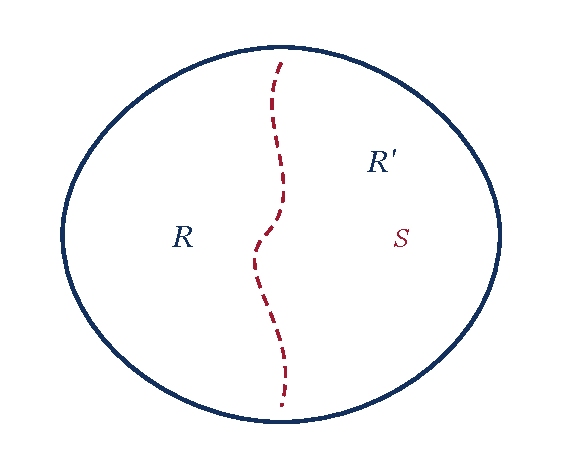
\includegraphics[width=0.6\textwidth]{figuras/pdf/cap01-fig1.pdf}
\caption{Un volumen del medio elástico dividido en dos partes $\mathrm{R}$
y $\mathrm{R}'$ por una superficie interior $S$.}
\label{fig:cap1-1}
\end{figure}

Este último potencial es muy pequeño. En efecto, las moléculas que
reaccionan unas sobre otras deben estar a una distancia menor que el radio
de la esfera de actividad molecular; por consiguiente, las moléculas del
volumen $\mathrm{R}$ que actúan sobre las del volumen $\mathrm{R}'$, y las
moléculas del volumen $\mathrm{R}'$ que actúan sobre las del volumen
$\mathrm{R}$, estarán comprendidas en el interior de un volumen limitado
por dos superficies paralelas a la superficie de separación de
$\mathrm{R}$ y de $\mathrm{R}'$, y situadas a una distancia de esta
superficie igual al radio de actividad molecular. Este volumen será
despreciable respecto de $\mathrm{R}$ y de $\mathrm{R}'$, y, si admitimos
que el número de moléculas de un medio es proporcional al volumen que
ocupan, las moléculas de cada uno de los volúmenes $\mathrm{R}$ y
$\mathrm{R}'$ que reaccionan sobre las moléculas del otro volumen serán en
número despreciable respecto de las moléculas contenidas en $\mathrm{R}$ o
en $\mathrm{R}'$. Por consiguiente, el potencial debido a la acción de las
moléculas del volumen $\mathrm{R}$ sobre las del volumen $\mathrm{R}'$
podrá despreciarse frente a $\mathrm{V}$ y $\mathrm{V}'$; tendremos:
\[
\mathrm{U}'=\mathrm{V}+\mathrm{V}'.
\]

Este razonamiento subsiste, por lo demás, si se divide el volumen ocupado
por el medio elástico en un número infinitamente grande de volúmenes
infinitamente pequeños, con tal de que las dimensiones de estos volúmenes
elementales sigan siendo infinitamente grandes respecto del radio de
actividad molecular; esto será siempre posible, puesto que este radio es un
infinitamente pequeño en valor absoluto. Designando por $d\tau$ uno de
estos elementos de volumen, por $\mathrm{W}\,d\tau$ el potencial debido a
las acciones mutuas de las moléculas situadas en el interior de este
elemento, el potencial de las fuerzas interiores del volumen total será:
\begin{equation}
\mathrm{U}'=\int \mathrm{W}\,d\tau.
\tag{16}
\end{equation}

\noindent\textbf{13.} Podemos desarrollar $\mathrm{W}$ según las potencias
crecientes de las $\xi$ y, despreciando los términos de grado superior al
segundo, tendremos:
\[
\mathrm{W}=\mathrm{W}_0+\mathrm{W}_1+\mathrm{W}_2.
\]
El término constante $\mathrm{W}_0$ puede suponerse nulo, y la relación
(16) nos dará:
\begin{equation}
\mathrm{U}'_1=\int \mathrm{W}_1\,d\tau,
\tag{17}
\end{equation}
\begin{equation}
\mathrm{U}'_2=\int \mathrm{W}_2\,d\tau.
\tag{18}
\end{equation}
La función de fuerzas $\mathrm{U}$ que entra en las ecuaciones del
movimiento se convertirá, teniendo en cuenta la relación (7), en:
\begin{equation}
\mathrm{U}=\mathrm{U}''_2+\int \mathrm{W}_2\,d\tau.
\tag{19}
\end{equation}

También podemos desarrollar la función $\mathrm{W}$ según las potencias
crecientes de las $\rho$, como lo hicimos para la función $\mathrm{U}'$; y,
remitiéndonos a la fórmula (15), escribiremos:
\begin{equation}
\mathrm{W}_2=\sum\frac{d\mathrm{F}}{d\mathrm{R}}\rho_2
+\frac12\sum\frac{d^2\mathrm{F}}{d\mathrm{R}^2}\rho_1^2
+\sum\frac{d^2\mathrm{F}}{d\mathrm{R}\,d\mathrm{R}'}\rho_1\rho_1',
\tag{20}
\end{equation}
extendiéndose la suma únicamente a las moléculas del elemento $d\tau$.
Siendo la cantidad $\rho_1$ homogénea y lineal respecto de las cantidades
$\mathrm{D}\xi,\mathrm{D}\eta,\mathrm{D}\zeta$, y $\rho_2$ homogénea y de
segundo grado respecto de esas mismas cantidades, resulta de la expresión
precedente que $\mathrm{W}_2$ es una función homogénea y de segundo grado
de $\mathrm{D}\xi,\mathrm{D}\eta,\mathrm{D}\zeta$.

\noindent\textbf{14. Nuevas hipótesis.} — Admitiremos que los
desplazamientos $\xi,\eta,\zeta$ son funciones continuas de las coordenadas
$x,y,z$ de la molécula en la posición de equilibrio, y que lo mismo ocurre
con sus derivadas sucesivas. Esta hipótesis es legítima, pues, si fuera de
otro modo, y si el desplazamiento relativo de dos moléculas muy vecinas no
fuera muy pequeño, resultarían de ello reacciones elásticas muy
considerables que no permitirían subsistir un estado de cosas semejante.

Admitida la continuidad de las funciones $\xi,\eta,\zeta$ y de sus
derivadas, podemos desarrollar estas funciones según las potencias
crecientes de las variables $x,y,z$, y tendremos:
\[
\mathrm{D}\xi=\frac{d\xi}{dx}\mathrm{D}x+\frac{d\xi}{dy}\mathrm{D}y+\frac{d\xi}{dz}\mathrm{D}z
+\frac12\left[\frac{d^2\xi}{dx^2}\mathrm{D}x^2+\frac{d^2\xi}{dy^2}\mathrm{D}y^2+\ldots\right]\ldots
\]
Las cantidades $\mathrm{D}x,\mathrm{D}y,\mathrm{D}z$, que son los
incrementos de las coordenadas al pasar de una molécula a una molécula
vecina, son del orden del radio de actividad molecular; los cuadrados de
estas cantidades serán infinitamente pequeños que en general se podrán
suprimir. Veremos sin embargo que no siempre tenemos el derecho de hacer
desaparecer estos cuadrados, y que una de las teorías propuestas para la
explicación de la dispersión de la luz necesita su conservación.
Suprimiéndolos, $\mathrm{D}\xi,\mathrm{D}\eta,\mathrm{D}\zeta$ vienen dados
por funciones lineales y homogéneas de las nueve derivadas parciales
\[
\frac{d\xi}{dx},\;\frac{d\xi}{dy},\;\frac{d\xi}{dz},\;\frac{d\eta}{dx},\ldots
\]
Se tiene:
\begin{equation}
\begin{gathered}
\mathrm{D}\xi=\frac{d\xi}{dx}\mathrm{D}x+\frac{d\xi}{dy}\mathrm{D}y+\frac{d\xi}{dz}\mathrm{D}z,\\
\mathrm{D}\eta=\frac{d\eta}{dx}\mathrm{D}x+\frac{d\eta}{dy}\mathrm{D}y+\frac{d\eta}{dz}\mathrm{D}z,\\
\mathrm{D}\zeta=\frac{d\zeta}{dx}\mathrm{D}x+\frac{d\zeta}{dy}\mathrm{D}y+\frac{d\zeta}{dz}\mathrm{D}z.
\end{gathered}
\tag{21}
\end{equation}

\noindent\textbf{15. Estudio de la función $\mathrm{W}_2$.} — Hemos visto
(§13) que $\mathrm{W}_2$ era una función homogénea de segundo grado
respecto a las cantidades $\mathrm{D}\xi,\mathrm{D}\eta,\mathrm{D}\zeta$;
es, pues, también una función homogénea y de segundo orden respecto a las
nueve derivadas parciales $\dfrac{d\xi}{dx},\dfrac{d\xi}{dy},\ldots$,
derivadas que en adelante representaremos a menudo con la notación de
Lagrange: $\xi'_x,\xi'_y,\xi'_z,\ldots$. Una forma cuadrática con nueve
variables independientes contiene nueve términos cuadrados y un número de
términos rectangulares igual al número de combinaciones de nueve objetos
tomados de dos en dos: $\dfrac{9\times 8}{2}=36$; puede, pues, contener
cuarenta y cinco coeficientes arbitrarios. Vamos a buscar el número de
coeficientes de la función $\mathrm{W}_2$.

Consideremos primero el término $\displaystyle\sum\frac{d\mathrm{F}}{d\mathrm{R}}\rho_2$
de esta función, desarrollado según la fórmula (20). Los términos en
$\xi_x'^2$ que entran en $\displaystyle\sum\frac{d\mathrm{F}}{d\mathrm{R}}\rho_2$
solo pueden provenir de $\mathrm{D}\xi^2$, pues ni $\mathrm{D}\eta$ ni
$\mathrm{D}\zeta$ contienen $\xi'_x$. Ahora bien, se tiene, elevando al
cuadrado los dos miembros de la primera de las relaciones (21):
\[
\mathrm{D}\xi^2=\left(\frac{d\xi}{dx}\right)^2\mathrm{D}x^2
+\left(\frac{d\xi}{dy}\right)^2\mathrm{D}y^2+\left(\frac{d\xi}{dz}\right)^2\mathrm{D}z^2
+2\frac{d\xi}{dx}\frac{d\xi}{dy}\mathrm{D}x\,\mathrm{D}y+\ldots;
\]
y el coeficiente de $\xi_x'^2$ en $\displaystyle\sum\frac{d\mathrm{F}}{d\mathrm{R}}\rho_2$ es:
\[
\sum\frac{d\mathrm{F}}{d\mathrm{R}}\mathrm{D}x^2.
\]
Se encontraría la misma cantidad para el coeficiente de $\eta_x'^2$ y de
$\zeta_x'^2$. Los coeficientes de los cuadrados de las nueve derivadas
parciales se reducen, pues, a tres:
\[
\sum\frac{d\mathrm{F}}{d\mathrm{R}}\mathrm{D}x^2,\qquad
\sum\frac{d\mathrm{F}}{d\mathrm{R}}\mathrm{D}y^2,\qquad
\sum\frac{d\mathrm{F}}{d\mathrm{R}}\mathrm{D}z^2.
\]
El coeficiente del doble producto $2\dfrac{d\xi}{dx}\dfrac{d\xi}{dy}$ es
$\displaystyle\sum\frac{d\mathrm{F}}{d\mathrm{R}}\mathrm{D}x\,\mathrm{D}y$.
Es fácil ver, desarrollando los cuadrados de $\mathrm{D}\eta$ y de
$\mathrm{D}\zeta$, que los productos $2\dfrac{d\eta}{dx}\dfrac{d\eta}{dy}$,
$2\dfrac{d\zeta}{dx}\dfrac{d\zeta}{dy}$, tienen por coeficientes esta misma
cantidad. Los coeficientes de los nueve dobles productos que entran en
$\displaystyle\sum\frac{d\mathrm{F}}{d\mathrm{R}}\rho_2$ se reducen, pues, a
los tres siguientes:
\[
\sum\frac{d\mathrm{F}}{d\mathrm{R}}\mathrm{D}x\,\mathrm{D}y,\qquad
\sum\frac{d\mathrm{F}}{d\mathrm{R}}\mathrm{D}y\,\mathrm{D}z,\qquad
\sum\frac{d\mathrm{F}}{d\mathrm{R}}\mathrm{D}z\,\mathrm{D}x.
\]
Por consiguiente, el primer término de $\mathrm{W}_2$ no contiene más que
seis coeficientes arbitrarios. Estos seis coeficientes son nulos cuando se
supone la presión exterior nula en el estado de equilibrio, según lo
establecido en el §10.

\noindent\textbf{16.} Los dos últimos términos de $\mathrm{W}_2$ son
homogéneos en $\rho_1$ y $\rho_1'$. Reemplazando, en la expresión de
$\rho_1$,
\[
\rho_1=2(\mathrm{D}x\,\mathrm{D}\xi+\mathrm{D}y\,\mathrm{D}\eta+\mathrm{D}z\,\mathrm{D}\zeta),
\]
$\mathrm{D}\xi,\mathrm{D}\eta,\mathrm{D}\zeta$ por sus valores (21), se
encuentra:
\begin{equation}
\begin{split}
\tfrac12\rho_1={}&\frac{d\xi}{dx}\mathrm{D}x^2+\frac{d\eta}{dy}\mathrm{D}y^2+\frac{d\zeta}{dz}\mathrm{D}z^2
+\left(\frac{d\xi}{dy}+\frac{d\eta}{dx}\right)\mathrm{D}x\,\mathrm{D}y\\
&+\left(\frac{d\eta}{dz}+\frac{d\zeta}{dy}\right)\mathrm{D}y\,\mathrm{D}z
+\left(\frac{d\zeta}{dx}+\frac{d\xi}{dz}\right)\mathrm{D}z\,\mathrm{D}x;
\end{split}
\tag{22}
\end{equation}
es decir, que $\rho_1$ es una función lineal y homogénea de las seis
cantidades
\[
\frac{d\xi}{dx},\quad \frac{d\eta}{dy},\quad \frac{d\zeta}{dz},\quad
\frac{d\xi}{dy}+\frac{d\eta}{dx},\quad \frac{d\eta}{dz}+\frac{d\zeta}{dy},\quad
\frac{d\zeta}{dx}+\frac{d\xi}{dz}.
\]
La suma de los dos últimos términos de $\mathrm{W}_2$
es, pues, una función homogénea y de segundo grado de estas seis
cantidades; por consiguiente, no contendrá más que $21$ coeficientes
arbitrarios ($6$ coeficientes para los cuadrados y $15$ para los dobles
productos).

\noindent\textbf{17.} Vemos ya que, en el caso más general, la función $\mathrm{W}_2$ no
contendrá más que $21+6=27$ coeficientes arbitrarios, número que se
reducirá a $21$ cuando la presión exterior sea nula en el estado de
equilibrio.

En la hipótesis de las fuerzas centrales, hemos visto (§11) que se tenía:
\[
\frac{d^2\mathrm{F}}{d\mathrm{R}\,d\mathrm{R}'}=0.
\]
El tercer término del desarrollo (20) de $\mathrm{W}_2$ desaparece
entonces, y, si en el segundo término reemplazamos $\rho_1^2$ por su valor
tomado de la relación (22), se comprueba que, entre los 21 coeficientes,
seis son iguales dos a dos. Así se tiene:
\[
\text{coef. de }\left(\frac{d\xi}{dy}+\frac{d\eta}{dx}\right)^2
=\text{coef. de }2\frac{d\xi}{dx}\frac{d\eta}{dy},
\]
\[
\text{coef. de }2\frac{d\zeta}{dz}\left(\frac{d\xi}{dy}+\frac{d\eta}{dx}\right)
=\text{coef. de }2\left(\frac{d\eta}{dz}+\frac{d\zeta}{dy}\right)\left(\frac{d\zeta}{dx}+\frac{d\xi}{dz}\right).
\]
El número de coeficientes arbitrarios se encuentra entonces reducido a 15.

En resumen, tendremos en $\mathrm{W}_2$: 1.\textsuperscript{o} 27
coeficientes arbitrarios en el caso general; 2.\textsuperscript{o} 21
coeficientes cuando la presión exterior es nula en el estado de equilibrio
y las fuerzas no son centrales; 3.\textsuperscript{o} 21 coeficientes
cuando las fuerzas son centrales y la presión exterior es distinta de cero
en el estado de equilibrio (hipótesis de Cauchy); 4.\textsuperscript{o} 15
coeficientes cuando las fuerzas son centrales y la presión exterior es
nula en el estado de equilibrio.

El valor de estos coeficientes, en un medio cualquiera, dependerá en
general de las coordenadas del centro de gravedad del elemento de volumen
$d\tau$. Para simplificar la cuestión y situarnos en el caso más corriente,
supondremos el medio homogéneo: los coeficientes se convertirán en
constantes.

\section{Funciones isótropas}

\noindent\textbf{18.} Un medio homogéneo se dice isótropo cuando, en ese
medio, todas las direcciones son idénticas. El éter en el vacío, los
cuerpos gaseosos, los líquidos, los sólidos amorfos son isótropos; los
sólidos cristalizados no lo son. De esta definición resulta que, en un
cuerpo isótropo, un plano cualquiera es un plano de simetría; en
particular, los planos de coordenadas son planos de simetría. Las
ecuaciones del movimiento y, por consiguiente, la función $\mathrm{W}_2$,
no deben cambiar cuando se sustituye $-x$ en lugar de $x$ y $-\xi$ en
lugar de $\xi$, o $-y$ en lugar de $y$ y $-\eta$ en lugar de $\eta$, o
finalmente $-z$ en lugar de $z$ y $-\zeta$ en lugar de $\zeta$.
Observaremos, por lo demás, que los cuerpos isótropos no son los únicos
que gozan de esta propiedad; pertenece a todos los cuerpos cristalizados
que poseen tres planos de simetría rectangulares, es decir, a los cuerpos
cristalizados pertenecientes a los cuatro primeros sistemas cristalinos.
Para estos cuerpos y para los isótropos, la función $\mathrm{W}_2$ no debe
contener términos que cambien de signo por alguna de las tres sustituciones
precedentes; es fácil reconocer que los términos que pueden subsistir
forman cuatro grupos: 1.\textsuperscript{o} los términos cuadrados de la
forma $\dfrac{d\xi^2}{dx^2}$; 2.\textsuperscript{o} los de la forma $\dfrac{d\xi^2}{dy^2}$;
3.\textsuperscript{o} los términos rectangulares tales como
$\dfrac{d\xi}{dx}\dfrac{d\eta}{dy}$; 4.\textsuperscript{o} el término
$\dfrac{d\xi}{dy}\dfrac{d\eta}{dx}$ y los que de él se deducen por
permutación.

Dentro de los cuerpos isótropos y de los cuerpos cristalizados del sistema
cúbico, todos los términos de un mismo grupo tienen el mismo coeficiente.
En efecto, en esos cuerpos las tres direcciones de los ejes de coordenadas
desempeñan el mismo papel; por consiguiente, podemos permutar dos de los
ejes, o los tres ejes, sin cambiar $\mathrm{W}_2$, es decir que
$\mathrm{W}_2$ debe conservar el mismo valor cuando en ella se permutan,
por ejemplo, $x$ e $y$, $\xi$ y $\eta$. Para que así sea, es necesario que
los coeficientes de los términos $\dfrac{d\xi^2}{dx^2},\dfrac{d\eta^2}{dy^2},
\dfrac{d\zeta^2}{dz^2}$ sean los mismos; por consiguiente, los términos del
primer grupo entran en la función $\mathrm{W}_2$ por su suma:
\[
\frac{d\xi^2}{dx^2}+\frac{d\eta^2}{dy^2}+\frac{d\zeta^2}{dz^2}.
\]
Como ocurre lo mismo para los términos de los otros tres grupos, la función
$\mathrm{W}_2$ es la suma de cuatro polinomios, homogéneos y de segundo
grado respecto a las nueve derivadas parciales, multiplicados
respectivamente por coeficientes numéricos. Estos cuatro polinomios son:
\[
\xi_x'^2+\eta_y'^2+\zeta_z'^2
\]
\[
\xi_y'^2+\xi_z'^2+\eta_x'^2+\eta_z'^2+\zeta_x'^2+\zeta_y'^2
\]
\[
\xi_x'\eta_y'+\xi_x'\zeta_z'+\eta_y'\zeta_z'
\]
\[
\xi_y'\eta_x'+\xi_z'\zeta_x'+\eta_z'\zeta_y'.
\]

\noindent\textbf{19.} Queda por averiguar si estos cuatro polinomios
independientes subsistirán en el caso de un cuerpo perfectamente isótropo.
Vamos a mostrar que se reducen a tres, que llamaremos polinomios isótropos.

Puesto que en un cuerpo isótropo todas las direcciones son idénticas, la
expresión de un polinomio isótropo no debe cambiar cuando se hace un cambio
cualquiera de coordenadas conservando el mismo origen; la forma de un
polinomio isótropo debe ser independiente de la elección de los ejes.

Sean $x,y,z$ las coordenadas de una molécula $\mu$ (figura~\ref{fig:cap1-2})
de un medio isótropo; $x+\mathrm{D}x,\,y+\mathrm{D}y,\,z+\mathrm{D}z$ las de
una molécula vecina $\mu'$. Cuando la molécula $\mu$ sea desplazada de su
posición de equilibrio, vendrá a $\mu_1$, cuyas coordenadas son
$x+\xi,\,y+\eta,\,z+\zeta$; la molécula $\mu'$ ocupará el punto $\mu'_1$ de
coordenadas $x+\xi+\mathrm{D}x+\mathrm{D}\xi,\,y+\eta+\mathrm{D}y+\mathrm{D}\eta,
\,z+\zeta+\mathrm{D}z+\mathrm{D}\zeta$. Por el punto $\mu$ tracemos la recta
$\mu\mu''$ igual y paralela a $\mu_1\mu'_1$, y unamos $\mu'$ a $\mu''$. Por
el punto $\mathrm{O}$, origen de las coordenadas, tracemos una recta
$\mathrm{OM}$ igual y paralela a $\mu\mu'$ y una recta $\mathrm{OP}$ igual y
paralela a $\mu'\mu''$; las coordenadas del punto $\mathrm{M}$ serán
$\mathrm{D}x,\mathrm{D}y,\mathrm{D}z$; las del punto $\mathrm{P}$ serán
$\mathrm{D}\xi,\mathrm{D}\eta,\mathrm{D}\zeta$.

\begin{figure}[h]
\centering
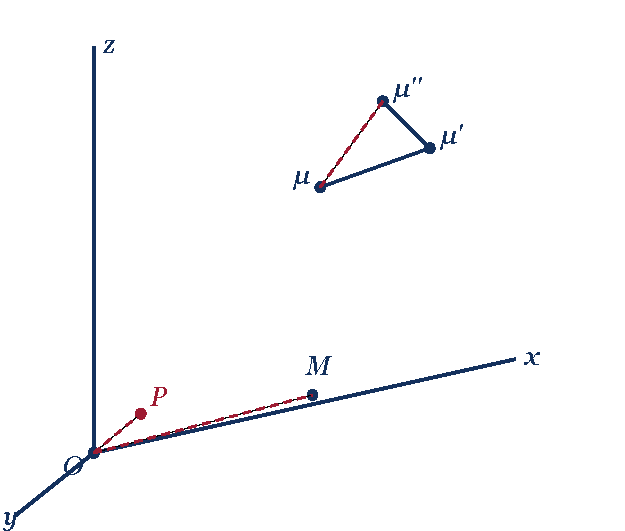
\includegraphics[width=0.75\textwidth]{figuras/pdf/cap01-fig2.pdf}
\caption{Construcción geométrica del §19: los puntos $\mu,\mu',\mu''$ y los
segmentos $\mathrm{OM}$, $\mathrm{OP}$, iguales y paralelos a $\mu\mu'$ y
$\mu'\mu''$.}
\label{fig:cap1-2}
\end{figure}

Designando por $l$ la longitud de la recta $\mathrm{OP}$, tendremos:
\begin{equation}
l^2=\mathrm{D}\xi^2+\mathrm{D}\eta^2+\mathrm{D}\zeta^2,
\tag{23}
\end{equation}
y, como, según las ecuaciones (21), $\mathrm{D}\xi,\mathrm{D}\eta,\mathrm{D}\zeta$
son funciones homogéneas y de primer grado respecto a $\mathrm{D}x,\mathrm{D}y,
\mathrm{D}z$, $l^2$ es una función homogénea y de segundo grado respecto a
las coordenadas del punto $\mathrm{M}$. Por consiguiente, el lugar de los
puntos $\mathrm{M}$ tales que la longitud $\mathrm{OP}$ permanezca
constante es un elipsoide cuyo centro está en $\mathrm{O}$. Siendo isótropo
el medio, debe encontrarse el mismo elipsoide cualquiera que sea la
dirección de los ejes. La ecuación del elipsoide dependerá naturalmente de
la elección de los ejes; pero el elipsoide mismo no cambiará cuando se
cambien los tres planos de coordenadas. Ahora bien, se sabe que, si un
elipsoide es fijo en el espacio, existen ciertas funciones de los
coeficientes de su ecuación, conocidas con el nombre de invariantes, que
son independientes de la elección de los ejes; ellas deberán ser funciones
isótropas. Uno de los invariantes es la suma de los cuadrados de los
coeficientes de los términos cuadrados. Para hallarlo, reemplacemos en la
ecuación (23) las cantidades $\mathrm{D}\xi,\mathrm{D}\eta,\mathrm{D}\zeta$
por los valores (21). Tendremos entre las coordenadas $\mathrm{D}x,\mathrm{D}y,
\mathrm{D}z$ del punto $\mathrm{M}$ una relación que será precisamente la
ecuación de nuestro elipsoide, y obtendremos para el coeficiente de
$\mathrm{D}x^2$ la suma:
\[
\xi_x'^2+\eta_x'^2+\zeta_x'^2;
\]
el de $\mathrm{D}y^2$ será:
\[
\xi_y'^2+\eta_y'^2+\zeta_y'^2;
\]
y el de $\mathrm{D}z^2$:
\[
\xi_z'^2+\eta_z'^2+\zeta_z'^2.
\]
La suma de estos tres coeficientes será, pues, una función isótropa. La
designaremos por $\mathrm{H}$; será la suma de los cuadrados de las nueve
derivadas parciales:
\begin{equation}
\mathrm{H}=\sum \xi_x'^2.
\tag{24}
\end{equation}

\noindent\textbf{20.} Para hallar otras funciones isótropas, consideremos
el caso en que las moléculas $\mu$ y $\mu'$ se desplazan de manera que la
recta $\mu\mu'$ permanezca siempre paralela a sí misma: las rectas
$\mathrm{OP}$ y $\mathrm{OM}$ son paralelas, y, designando por $\alpha$ la
razón de sus longitudes, se tiene:
\[
\mathrm{D}\xi=\alpha\,\mathrm{D}x,\qquad \mathrm{D}\eta=\alpha\,\mathrm{D}y,
\qquad \mathrm{D}\zeta=\alpha\,\mathrm{D}z.
\]
Si se llevan estos valores a las ecuaciones (21) del §14, se obtiene:
\[
\alpha\,\mathrm{D}x=\xi_x'\,\mathrm{D}x+\xi_y'\,\mathrm{D}y+\xi_z'\,\mathrm{D}z,
\]
\[
\alpha\,\mathrm{D}y=\eta_x'\,\mathrm{D}x+\eta_y'\,\mathrm{D}y+\eta_z'\,\mathrm{D}z,
\]
\[
\alpha\,\mathrm{D}z=\zeta_x'\,\mathrm{D}x+\zeta_y'\,\mathrm{D}y+\zeta_z'\,\mathrm{D}z,
\]
y la eliminación de $\mathrm{D}x,\mathrm{D}y,\mathrm{D}z$ entre estas
ecuaciones conduce al determinante:
\[
\begin{vmatrix}
\xi_x'-\alpha & \xi_y' & \xi_z'\\
\eta_x' & \eta_y'-\alpha & \eta_z'\\
\zeta_x' & \zeta_y' & \zeta_z'-\alpha
\end{vmatrix}=0.
\]
Esta ecuación determinará $\alpha$. Ahora bien, esta cantidad es
evidentemente independiente de la elección de los ejes de coordenadas; por
consiguiente, los coeficientes de esta ecuación en $\alpha$ son
invariantes. El coeficiente del término en $\alpha^2$ es:
\[
\xi_x'+\eta_y'+\zeta_z'.
\]
Designaremos esta nueva función isótropa por $\Theta$, y, como entrará en
segundo grado en la función $\mathrm{W}_2$, consideraremos su cuadrado:
\begin{equation}
\Theta^2=(\xi_x'+\eta_y'+\zeta_z')^2.
\tag{25}
\end{equation}

\noindent\textbf{21.} Esta función $\Theta$ tiene una significación
geométrica interesante.

El volumen de una porción del medio elástico en su posición de equilibrio
tiene por expresión:
\[
\iiint dx\,dy\,dz.
\]
A causa de la deformación del medio, las coordenadas del centro de
gravedad de cada elemento del volumen se convierten en $x+\xi,\,y+\eta,
\,z+\zeta$, y el volumen de la porción considerada toma el valor:
\[
\iiint (dx+d\xi)(dy+d\eta)(dz+d\zeta).
\]
Recordemos que, si se tiene una integral
\[
\iiint \mathrm{F}(x,y,z)\,dx\,dy\,dz
\]
donde $x,y,z$ son funciones de tres nuevas variables $\alpha,\beta,\gamma$,
esta integral se convierte, al tomar como variables $\alpha,\beta,\gamma$,
en
\[
\iiint \Phi(\alpha,\beta,\gamma)\,\frac{\mathrm{D}(x,y,z)}{\mathrm{D}(\alpha,\beta,\gamma)}\,d\alpha\,d\beta\,d\gamma,
\]
designando $\mathrm{D}(x,y,z)/\mathrm{D}(\alpha,\beta,\gamma)$ el
determinante funcional\footnote{Es lo que hoy se llama el \emph{jacobiano}
de $x,y,z$ respecto a $\alpha,\beta,\gamma$.} de $x,y,z$ respecto a
$\alpha,\beta,\gamma$. Apoyándonos en este teorema, tendremos,
para la expresión del volumen después de la deformación:
\[
\iiint \frac{\mathrm{D}[(x+\xi),(y+\eta),(z+\zeta)]}{\mathrm{D}(x,y,z)}\,dx\,dy\,dz.
\]
El determinante funcional que entra en esta integral tiene por valor:
\[
\begin{vmatrix}
1+\xi_x' & \xi_y' & \xi_z'\\
\eta_x' & 1+\eta_y' & \eta_z'\\
\zeta_x' & \zeta_y' & 1+\zeta_z'
\end{vmatrix}
\]
y, si, en el desarrollo de este determinante, se desprecian las potencias
de las derivadas que son superiores al primer grado, se obtiene:
\[
1+\xi_x'+\eta_y'+\zeta_z',
\]
es decir:
\[
1+\Theta.
\]
Si llevamos este valor del determinante funcional a la integral que da el
volumen después de la deformación, obtenemos:
\[
\iiint (1+\Theta)\,dx\,dy\,dz.
\]
Un elemento de volumen $dx\,dy\,dz$ se convierte, pues, después de la
deformación, en $(1+\Theta)\,dx\,dy\,dz$; por consiguiente, $\Theta$ es el
coeficiente de dilatación cúbica del medio.

\noindent\textbf{22.} Volvamos a nuestra ecuación en $\alpha$. El
coeficiente del término en $-\alpha$ es:
\begin{equation}
\mathrm{K}=\xi_x'\eta_y'-\xi_y'\eta_x'+\eta_y'\zeta_z'-\eta_z'\zeta_y'+\zeta_z'\xi_x'-\zeta_x'\xi_z'.
\tag{26}
\end{equation}
Es un tercer polinomio isótropo, que puede escribirse:
\[
\mathrm{K}=\frac{\mathrm{D}(\xi,\eta)}{\mathrm{D}(x,y)}+\frac{\mathrm{D}(\eta,\zeta)}{\mathrm{D}(y,z)}+\frac{\mathrm{D}(\zeta,\xi)}{\mathrm{D}(z,x)}.
\]

\noindent\textbf{23.} Los tres polinomios isótropos de segundo grado,
$\mathrm{H},\Theta^2,\mathrm{K}$, son tres polinomios independientes. No
puede haber otros, pues, si hubiera cuatro, todos los cuerpos que gozan de
la simetría cúbica —para la cual la función $\mathrm{W}_2$ es una suma de
cuatro polinomios de segundo grado e independientes— gozarían al mismo
tiempo de la isotropía. Por lo demás, el primero de los polinomios que
entra en $\mathrm{W}_2$, en el caso de los cuerpos de simetría cúbica (§18):
\[
\xi_x'^2+\eta_y'^2+\zeta_z'^2
\]
no es un polinomio isótropo, pues cambia cuando se hacen girar los ejes,
como es fácil convencerse haciendo girar los ejes de las $x$ y de las $y$
en $45^\circ$ en el plano de las $xy$.

\section{Expresión de $\mathrm{W}_2$ en el caso de los cuerpos isótropos}

\noindent\textbf{24.} La función $\mathrm{W}_2$ no puede contener más que
los tres polinomios isótropos que acabamos de hallar, y, como esta función
es homogénea y de segundo grado respecto a las nueve derivadas parciales
$\xi_x',\xi_y',\ldots$, debe ser lineal y homogénea respecto a los tres
polinomios isótropos, que son ellos mismos homogéneos y de segundo grado
respecto a las nueve derivadas parciales; será de la forma:
\begin{equation}
\mathrm{W}_2=\lambda\mathrm{K}+\mu\mathrm{H}+\nu\Theta^2.
\tag{27}
\end{equation}

Comparemos esta expresión con el desarrollo (20) de esta misma función. El
primer término de este desarrollo y el conjunto de los dos últimos deberán
ser separadamente isótropos, pues, en un medio isótropo, toda función
simétrica de las distancias mutuas de los puntos ocupados por las
moléculas antes y después del desplazamiento debe ser una función isótropa.

Consideremos primero el término $\displaystyle\sum\frac{d\mathrm{F}}{d\mathrm{R}}\rho_2$
de esta expresión; vamos a demostrar que es igual al polinomio $\mathrm{H}$
multiplicado por un factor constante.

En el estudio de la función $\mathrm{W}_2$ (§15) hemos visto que, si
reemplazamos en el primer término del desarrollo de esta función las
cantidades $\mathrm{D}\xi,\mathrm{D}\eta,\mathrm{D}\zeta$ por sus valores
dados por las relaciones (21), obtenemos para este término un polinomio
homogéneo y de segundo grado respecto a las nueve derivadas parciales,
que contiene los cuadrados de estas derivadas y los nueve dobles productos
de la forma $\dfrac{d\xi}{dx}\dfrac{d\xi}{dy}$. Pero este término, siendo
una función isótropa, no puede contener esos dobles productos, que no
entran en ninguno de los cuatro grupos de términos que subsisten en el caso
de los cuerpos de simetría cúbica (§18); el primer término de $\mathrm{W}_2$
se reduce, pues, a un polinomio que no contiene más que los cuadrados de
las derivadas parciales. No puede contener ni $\Theta$ ni $\mathrm{K}$,
pues en la función $\mathrm{K}$ se encuentran dobles productos tales como
$\xi_y'\eta_x'$ que no pueden reducirse con los dobles productos de
$\Theta^2$, que no son de esta forma. Debemos, pues, tener:
\begin{equation}
\sum\frac{d\mathrm{F}}{d\mathrm{R}}\rho_2=\mu_1\mathrm{H}.
\tag{28}
\end{equation}

\noindent\textbf{25.} El conjunto de los dos últimos términos:
\[
\frac12\sum\frac{d^2\mathrm{F}}{d\mathrm{R}^2}\rho_1^2
+\sum\frac{d^2\mathrm{F}}{d\mathrm{R}\,d\mathrm{R}'}\rho_1\rho_1'
\]
del desarrollo (20) de la función $\mathrm{W}_2$ es también, en el caso de
los cuerpos isótropos, una función isótropa, y de las relaciones (20) (27)
y (28) deducimos la igualdad:
\begin{equation}
\frac12\sum\frac{d^2\mathrm{F}}{d\mathrm{R}^2}\rho_1^2
+\sum\frac{d^2\mathrm{F}}{d\mathrm{R}\,d\mathrm{R}'}\rho_1\rho_1'
=\lambda\mathrm{K}+(\mu-\mu_1)\mathrm{H}+\nu\Theta^2.
\tag{29}
\end{equation}

En el estudio de la función $\mathrm{W}_2$ (§16) hemos mostrado que, en
el caso general, el primer miembro de esta igualdad es una función homogénea y de segundo
grado de las seis cantidades:
\[
\xi_x',\quad \eta_y',\quad \zeta_z',
\]
\[
\xi_y'+\eta_x',\quad \eta_z'+\zeta_y',\quad \zeta_x'+\xi_z'.
\]
Los términos $\xi_y'^2$ y $2\xi_y'\eta_x'$ solo pueden provenir del
cuadrado de la cantidad $\xi_y'+\eta_x'$; por consiguiente, estos términos
deben tener el mismo coeficiente. Ahora bien, el término $\xi_y'^2$ no se
encuentra más que en la función $\mathrm{H}$, donde tiene el coeficiente
$1$; entrará, pues, en el segundo miembro de la relación (29) con el
coeficiente $\mu-\mu_1$.

El término $2\xi_y'\eta_x'$ no puede provenir más que
de la función $\mathrm{K}$, donde tiene el coeficiente $-\tfrac12$; su
coeficiente, en el segundo miembro de (29), será, pues, $-\tfrac{\lambda}{2}$.
Teniendo los dos términos considerados el mismo coeficiente en el primer
miembro de la relación, debe ocurrir lo mismo en el segundo miembro; por
consiguiente tendremos:
\begin{equation}
\mu-\mu_1=-\frac{\lambda}{2}.
\tag{30}
\end{equation}

\noindent\textbf{26.} Cuando se supone que la presión exterior es nula en el estado de
equilibrio, el término $\displaystyle\sum\frac{d\mathrm{F}}{d\mathrm{R}}\rho_2$
del desarrollo (20) desaparece (§15); por consiguiente, $\mu_1$ es nulo, y
la relación precedente se convierte en:
\begin{equation}
\mu=-\frac{\lambda}{2}.
\tag{31}
\end{equation}
No queda entonces más que dos coeficientes arbitrarios en la función
$\mathrm{W}_2$.

En la hipótesis de las fuerzas centrales, el término
$\displaystyle\sum\frac{d^2\mathrm{F}}{d\mathrm{R}\,d\mathrm{R}'}\rho_1\rho_1'$
es nulo (§17), y el primer miembro de la relación (29) se reduce a
$\tfrac12\displaystyle\sum\frac{d^2\mathrm{F}}{d\mathrm{R}^2}\rho_1^2$.
Ahora bien, hemos visto que, si se reemplaza $\rho_1^2$ por su valor
tomado de la relación (22), se obtenía:
\[
\text{coef. de }\left(\frac{d\xi}{dy}+\frac{d\eta}{dx}\right)^2
=\text{coef. de }2\frac{d\xi}{dx}\frac{d\eta}{dy};
\]
por consiguiente, el coeficiente de $\xi_y'^2$ debe ser igual al de
$2\xi_x'\eta_y'$ en el primer miembro de la igualdad (29), y debe ocurrir
lo mismo en el segundo miembro. El término $\xi_y'^2$ se encuentra en él
con el coeficiente $\mu-\mu_1$; el término $2\xi_x'\eta_y'$, que entra en
$\Theta^2$ con el coeficiente $1$ y en $\mathrm{K}$ con el coeficiente
$\tfrac12$, está en el segundo miembro de (29) con el coeficiente
$\nu+\tfrac{\lambda}{2}$. Por consiguiente, se tiene la relación:
\[
\mu-\mu_1=\nu+\frac{\lambda}{2}.
\]
Reemplazando en ella $\mu-\mu_1$ por su valor dado por (30), se obtiene:
\begin{equation}
\lambda+\nu=0;
\tag{32}
\end{equation}
y el número de coeficientes arbitrarios se encuentra reducido a dos.

\noindent\textbf{27.} En resumen, la función $\mathrm{W}_2$ relativa a las
fuerzas interiores que resultan de la deformación de un medio isótropo es
una función homogénea y de segundo grado de las nueve derivadas de las
cantidades $\xi$, que contiene a lo más tres coeficientes arbitrarios
$\lambda,\mu,\nu$. El número de estos coeficientes puede reducirse, en
ciertos casos particulares; tendremos:

1.\textsuperscript{o} Tres coeficientes arbitrarios en el caso general;

2.\textsuperscript{o} Dos coeficientes cuando la presión exterior es nula
en el estado de equilibrio y las fuerzas no son centrales;

3.\textsuperscript{o} Dos coeficientes cuando las fuerzas son centrales y
la presión exterior es distinta de cero en el estado de equilibrio
(hipótesis de Cauchy);

4.\textsuperscript{o} Un solo coeficiente cuando las fuerzas son centrales
y la presión exterior es nula en el estado de equilibrio, pues, en este
caso, las relaciones (31) y (32) se verifican simultáneamente.

\section{Presiones exteriores. Ecuaciones del movimiento}

\noindent\textbf{28. Expresión de $\mathrm{W}_1$ en función de las
derivadas parciales.} — La función $\mathrm{W}_1$ es el término de primer
grado del desarrollo de la función $\mathrm{W}$ respecto a las potencias
crecientes de las $\xi$ (§13); esta última función puede, como la función
$\mathrm{U}'$, desarrollarse según las potencias crecientes de las $\rho$,
y, remitiéndonos a las relaciones (12) y (17), obtendremos:
\[
\mathrm{W}_1=\sum\frac{d\mathrm{F}}{d\mathrm{R}}\rho_1,
\]
extendiéndose la suma únicamente a las moléculas del elemento de volumen
$d\tau$. Reemplazando $\rho_1$ por su valor tomado de la relación (22), la
función $\mathrm{W}_1$ se convierte en:
\[
\frac12\mathrm{W}_1=\xi_x'\sum\frac{d\mathrm{F}}{d\mathrm{R}}\mathrm{D}x^2
+\eta_y'\sum\frac{d\mathrm{F}}{d\mathrm{R}}\mathrm{D}y^2
+\zeta_z'\sum\frac{d\mathrm{F}}{d\mathrm{R}}\mathrm{D}z^2
+(\xi_y'+\eta_x')\sum\frac{d\mathrm{F}}{d\mathrm{R}}\mathrm{D}x\,\mathrm{D}y+\ldots
\]
Es, pues, una función homogénea y de primer grado respecto a las nueve
derivadas parciales.

\noindent\textbf{29. Presiones exteriores. — Ecuaciones del movimiento.} —
Consideremos una superficie cerrada $S$ (figura~\ref{fig:cap1-1}) que
divide el medio elástico en dos partes: una, $\mathrm{R}$, interior a la
superficie; la otra, $\mathrm{R}'$, exterior. Las diversas moléculas de
$\mathrm{R}'$ ejercen acciones sobre las moléculas de $\mathrm{R}$, pero,
siendo muy pequeño el radio de la esfera de actividad molecular, solo las
moléculas de $\mathrm{R}$ vecinas de la superficie están sometidas a las
acciones de $\mathrm{R}'$. Estas acciones pueden reemplazarse por un
sistema de fuerzas aplicadas a los elementos $d\omega$ de la superficie
$S$ y que, en general, actuarán oblicuamente sobre el elemento
considerado. Designaremos por
\[
\mathrm{P}_x\,d\omega,\qquad \mathrm{P}_y\,d\omega,\qquad \mathrm{P}_z\,d\omega,
\]
las componentes según los tres ejes de la presión que se ejerce sobre el
elemento $d\omega$; son las fuerzas exteriores al sistema, si solo se
considera el volumen $\mathrm{R}$ limitado por la superficie. La aplicación
del principio de d'Alembert y del principio de las velocidades virtuales a
este sistema nos va a permitir hallar los valores de las componentes de las
presiones y, al mismo tiempo, darnos una nueva forma de las ecuaciones del
movimiento.

Si $\rho$ es la densidad de un elemento de volumen $d\tau$ (en adelante la
letra $\rho$ se empleará exclusivamente en este sentido), la masa del
elemento es $\rho\,d\tau$, y las tres componentes de la fuerza de inercia
que hay que suponer aplicada a este elemento, para que, según el principio
de d'Alembert, este elemento pueda considerarse en equilibrio, son:
\[
-\rho\,d\tau\,\frac{d^2\xi}{dt^2},\qquad -\rho\,d\tau\,\frac{d^2\eta}{dt^2},
\qquad -\rho\,d\tau\,\frac{d^2\zeta}{dt^2}.
\]
Estando todos los elementos del volumen $\mathrm{R}$ en equilibrio bajo la
acción de las fuerzas efectivas y de las fuerzas de inercia, se podrá
aplicar a este volumen el principio de las velocidades virtuales: en un
sistema en equilibrio, la suma de los trabajos virtuales es nula.
Designando por $\mathrm{U}$ la función de fuerzas relativa a las fuerzas
interiores y exteriores a $\mathrm{R}$, la suma de los trabajos virtuales
de estas fuerzas es $\delta\mathrm{U}$; y, llamando $\delta\xi,\delta\eta,
\delta\zeta$ a las proyecciones del desplazamiento virtual de un elemento
$d\tau$, el trabajo virtual de la fuerza de inercia es:
\[
-\rho\,d\tau\left(\frac{d^2\xi}{dt^2}\delta\xi+\frac{d^2\eta}{dt^2}\delta\eta+\frac{d^2\zeta}{dt^2}\delta\zeta\right).
\]
La suma de los trabajos de todas las fuerzas de inercia será:
\[
-\int \rho\,d\tau\left(\frac{d^2\xi}{dt^2}\delta\xi+\frac{d^2\eta}{dt^2}\delta\eta+\frac{d^2\zeta}{dt^2}\delta\zeta\right);
\]
y, según el principio de las velocidades virtuales, se tendrá:
\begin{equation}
\delta\mathrm{U}-\int \rho\,d\tau\left(\frac{d^2\xi}{dt^2}\delta\xi+\frac{d^2\eta}{dt^2}\delta\eta+\frac{d^2\zeta}{dt^2}\delta\zeta\right)=0,
\tag{33}
\end{equation}
cualesquiera que sean $\delta\xi,\delta\eta,\delta\zeta$.

Observemos que, según la relación (19), tenemos:
\[
\delta\mathrm{U}=\delta\mathrm{U}''+\int\delta\mathrm{W}\,d\tau;
\]
siendo $\delta\mathrm{U}''$ la suma de los trabajos virtuales de las
fuerzas exteriores, es decir, de las presiones definidas anteriormente,
tendremos:
\[
\delta\mathrm{U}''=\int d\omega\,(\mathrm{P}_x\,\delta\xi+\mathrm{P}_y\,\delta\eta+\mathrm{P}_z\,\delta\zeta),
\]
extendiéndose la integral a toda la superficie $S$. Si se supone que las
componentes $\delta\eta$ y $\delta\zeta$ del desplazamiento son nulas, el
trabajo virtual de las fuerzas exteriores se reduce a:
\[
\delta\mathrm{U}''=\int d\omega\,\mathrm{P}_x\,\delta\xi.
\]

La función $\mathrm{W}$ relativa a las fuerzas
interiores es una función de las nueve derivadas parciales de las $\xi$.
Por efecto del desplazamiento virtual dado al sistema, cada una de estas
derivadas varía en general, pero, en el caso particular donde se tiene
$\delta\eta=\delta\zeta=0$, las únicas derivadas que cambian de valor son
$\xi_x',\xi_y',\xi_z'$. Por consiguiente:
\[
\delta\mathrm{W}=\frac{d\mathrm{W}}{d\xi_x'}\delta\xi_x'+\frac{d\mathrm{W}}{d\xi_y'}\delta\xi_y'+\frac{d\mathrm{W}}{d\xi_z'}\delta\xi_z'
=\sum\frac{d\mathrm{W}}{d\xi_x'}\delta\xi_x'.
\]
Ahora bien, $\delta\xi_x'$, es decir $\delta\dfrac{d\xi}{dx}$, es igual a
$\dfrac{d}{dx}\delta\xi$, y la expresión de $\delta\mathrm{W}$ se convierte
en
\[
\delta\mathrm{W}=\sum\frac{d\mathrm{W}}{d\xi_x'}\frac{d}{dx}\delta\xi.
\]
Por consiguiente, se tiene:
\[
\delta\mathrm{U}=\int d\omega\,\mathrm{P}_x\,\delta\xi+\int d\tau\sum\frac{d\mathrm{W}}{d\xi_x'}\frac{d}{dx}\delta\xi,
\]
y, llevando este valor a la igualdad (33), donde se hace $\delta\eta=\delta\zeta=0$
en el término relativo a los trabajos de las fuerzas de inercia, se
obtiene:
\begin{equation}
\int d\omega\,\mathrm{P}_x\,\delta\xi+\int d\tau\sum\frac{d\mathrm{W}}{d\xi_x'}\frac{d}{dx}\delta\xi
-\int \rho\,d\tau\,\frac{d^2\xi}{dt^2}\,\delta\xi=0.
\tag{34}
\end{equation}

\noindent\textbf{30.} Hay que transformar ahora esta expresión, que
contiene a la vez $\delta\xi$ y la derivada de esta cantidad respecto a
$x$. Para ello nos apoyaremos en el siguiente lema, que sirve
ordinariamente para la demostración del teorema de Green en la teoría del
potencial:\footnote{Es el teorema de la divergencia (de
Gauss--Ostrogradski) escrito para una sola componente.} dada una función $\mathrm{F}$ de las coordenadas
$x,y,z$ de un punto, la integral de la diferencial $\mathrm{F}\alpha\,d\omega$,
donde $\alpha$ es el primer coseno director de la normal al elemento
$d\omega$ de una superficie cerrada $S$, extendida esta integral a todos
los elementos de la superficie $S$, es igual a la integral de la
diferencial $\dfrac{d\mathrm{F}}{dx}\,d\tau$, extendida a todos los
elementos $d\tau$ del volumen $\mathrm{R}$ limitado por la superficie $S$.

Si ponemos:
\[
\mathrm{F}=\frac{d\mathrm{W}}{d\xi_x'}\,\delta\xi,
\]
tendremos:
\[
\int \frac{d\mathrm{W}}{d\xi_x'}\,\alpha\,\delta\xi\,d\omega
=\int \frac{d\left(\dfrac{d\mathrm{W}}{d\xi_x'}\,\delta\xi\right)}{dx}\,d\tau;
\]
o, desarrollando la integral del segundo miembro:
\[
\int \frac{d\mathrm{W}}{d\xi_x'}\,\delta\xi\,\alpha\,d\omega
=\int \frac{d\dfrac{d\mathrm{W}}{d\xi_x'}}{dx}\,\delta\xi\,d\tau
+\int \frac{d\mathrm{W}}{d\xi_x'}\,\frac{d\,\delta\xi}{dx}\,d\tau.
\]
Obtendremos de la misma manera las dos relaciones:
\[
\int \frac{d\mathrm{W}}{d\xi_y'}\,\delta\xi\,\beta\,d\omega
=\int \frac{d\dfrac{d\mathrm{W}}{d\xi_y'}}{dy}\,\delta\xi\,d\tau
+\int \frac{d\mathrm{W}}{d\xi_y'}\,\frac{d\,\delta\xi}{dy}\,d\tau,
\]
\[
\int \frac{d\mathrm{W}}{d\xi_z'}\,\delta\xi\,\gamma\,d\omega
=\int \frac{d\dfrac{d\mathrm{W}}{d\xi_z'}}{dz}\,\delta\xi\,d\tau
+\int \frac{d\mathrm{W}}{d\xi_z'}\,\frac{d\,\delta\xi}{dz}\,d\tau.
\]
Sumando estas tres relaciones miembro a miembro, obtenemos:
\[
\int \delta\xi\,d\omega\sum\alpha\frac{d\mathrm{W}}{d\xi_x'}
=\int \delta\xi\,d\tau\sum\frac{d\dfrac{d\mathrm{W}}{d\xi_x'}}{dx}
+\int d\tau\sum\frac{d\mathrm{W}}{d\xi_x'}\frac{d\,\delta\xi}{dx},
\]
o
\[
\int d\tau\sum\frac{d\mathrm{W}}{d\xi_x'}\frac{d\,\delta\xi}{dx}
=\int \delta\xi\,d\omega\sum\alpha\frac{d\mathrm{W}}{d\xi_x'}
-\int \delta\xi\,d\tau\sum\frac{d\dfrac{d\mathrm{W}}{d\xi_x'}}{dx}.
\]
El primer miembro de esta relación es precisamente el término de la
igualdad (34) que contiene la derivada de $\delta\xi$; reemplacemos este
término por su valor, obtendremos:
\[
\int d\omega\,\mathrm{P}_x\,\delta\xi+\int \delta\xi\,d\omega\sum\alpha\frac{d\mathrm{W}}{d\xi_x'}
-\int \delta\xi\,d\tau\sum\frac{d\dfrac{d\mathrm{W}}{d\xi_x'}}{dx}
-\int \rho\,d\tau\,\frac{d^2\xi}{dt^2}\,\delta\xi=0;
\]
o, reuniendo bajo el mismo signo las cantidades que sufren la misma
integración:
\[
\int \delta\xi\,d\omega\left(\mathrm{P}_x+\sum\alpha\frac{d\mathrm{W}}{d\xi_x'}\right)
-\int \delta\xi\,d\tau\left(\rho\frac{d^2\xi}{dt^2}+\sum\frac{d\dfrac{d\mathrm{W}}{d\xi_x'}}{dx}\right)=0.
\]
Debiendo tener lugar esta igualdad cualquiera que sea $\delta\xi$, es
necesario que los coeficientes de $\delta\xi\,d\omega$ y de
$\delta\xi\,d\tau$ sean nulos; por consiguiente, tendremos:
\begin{equation}
\mathrm{P}_x=-\sum\alpha\frac{d\mathrm{W}}{d\xi_x'},
\tag{35}
\end{equation}
\begin{equation}
-\rho\frac{d^2\xi}{dt^2}=\sum\frac{d}{dx}\frac{d\mathrm{W}}{d\xi_x'}.
\tag{36}
\end{equation}

\noindent\textbf{31.} La primera de estas igualdades da el valor de la
componente de la presión según el eje $x$; poniendo
\[
-\frac{d\mathrm{W}}{d\xi_x'}=\mathrm{P}_{xx},\qquad
-\frac{d\mathrm{W}}{d\xi_y'}=\mathrm{P}_{xy},\qquad
-\frac{d\mathrm{W}}{d\xi_z'}=\mathrm{P}_{xz},
\]
la expresión de esta componente se convierte en:
\[
\mathrm{P}_x=\alpha\,\mathrm{P}_{xx}+\beta\,\mathrm{P}_{xy}+\gamma\,\mathrm{P}_{xz}.
\]
Consideremos una de las cantidades $\mathrm{P}_{xx}$ que entran en esta
expresión; se tiene:
\[
\mathrm{P}_{xx}=-\frac{d\mathrm{W}}{d\xi_x'}=-\frac{d\mathrm{W}_1}{d\xi_x'}-\frac{d\mathrm{W}_2}{d\xi_x'}.
\]
Ahora bien, $\mathrm{W}_1$ es una función lineal y homogénea de las
derivadas parciales, $\mathrm{W}_2$ una función de segundo grado de esas
mismas cantidades; luego el primer término de $\mathrm{P}_{xx}$ es una
constante y el segundo una función de primer grado de las derivadas
parciales. Cuando el medio está en su posición de equilibrio, las
cantidades $\xi$ son nulas y, siendo cero un mínimo para esas cantidades,
sus derivadas $\xi_x',\xi_y',\ldots$ son nulas también; el segundo término
de $\mathrm{P}_{xx}$ desaparece, y el valor de $\mathrm{P}_{xx}$ en la
posición de equilibrio es:
\[
\mathrm{P}_{xx}=-\frac{d\mathrm{W}_1}{d\xi_x'}.
\]
Si nos remitimos al valor de $\mathrm{W}_1$ que hemos hallado (§28), se ve
que:
\[
\mathrm{P}_{xx}=-2\sum\frac{d\mathrm{F}}{d\mathrm{R}}\mathrm{D}x^2.
\]
Se encontraría, para la posición de equilibrio del sistema, de la misma
manera:
\[
\mathrm{P}_{xy}=-2\sum\frac{d\mathrm{F}}{d\mathrm{R}}\mathrm{D}x\,\mathrm{D}y,
\qquad \mathrm{P}_{xz}=-2\sum\frac{d\mathrm{F}}{d\mathrm{R}}\mathrm{D}x\,\mathrm{D}z,\ldots
\]
Estas expresiones muestran que, si las seis cantidades
\[
\sum\frac{d\mathrm{F}}{d\mathrm{R}}\mathrm{D}x^2,\quad
\sum\frac{d\mathrm{F}}{d\mathrm{R}}\mathrm{D}y^2,\quad
\sum\frac{d\mathrm{F}}{d\mathrm{R}}\mathrm{D}z^2,
\]
\[
\sum\frac{d\mathrm{F}}{d\mathrm{R}}\mathrm{D}y\,\mathrm{D}z,\quad
\sum\frac{d\mathrm{F}}{d\mathrm{R}}\mathrm{D}z\,\mathrm{D}x,\quad
\sum\frac{d\mathrm{F}}{d\mathrm{R}}\mathrm{D}x\,\mathrm{D}y,
\]
son nulas, la presión exterior es nula en el estado de equilibrio. Es la
recíproca de la propiedad que hemos demostrado en el §10.

\noindent\textbf{32.} Consideremos ahora la ecuación (36), que es una de las ecuaciones del
movimiento; reemplazando en ella $\mathrm{W}$ por su desarrollo
$\mathrm{W}_1+\mathrm{W}_2$, se convierte en:
\[
-\rho\frac{d^2\xi}{dt^2}=\sum\frac{d}{dx}\frac{d\mathrm{W}_1}{d\xi_x'}
+\sum\frac{d}{dx}\frac{d\mathrm{W}_2}{d\xi_x'}.
\]
Siendo $\mathrm{W}_1$ lineal y homogénea respecto a las derivadas
parciales, $\dfrac{d\mathrm{W}_1}{d\xi_x'}$ es una constante; la derivada
de esta función respecto a $x$ es nula, y el primer término del segundo
miembro de la ecuación desaparece. Las ecuaciones del movimiento se
reducirán, pues, a:
\[
-\rho\frac{d^2\xi}{dt^2}=\sum\frac{d}{dx}\frac{d\mathrm{W}_2}{d\xi_x'},\qquad
-\rho\frac{d^2\eta}{dt^2}=\sum\frac{d}{dx}\frac{d\mathrm{W}_2}{d\eta_x'},\qquad
-\rho\frac{d^2\zeta}{dt^2}=\sum\frac{d}{dx}\frac{d\mathrm{W}_2}{d\zeta_x'}.
\]
\noindent\textbf{33. Ecuaciones del movimiento en los cuerpos isótropos.}
— En el caso de los cuerpos isótropos, la función $\mathrm{W}_2$ viene dada
por la relación (27) (§24):
\[
\mathrm{W}_2=\lambda\mathrm{K}+\mu\mathrm{H}+\nu\Theta^2.
\]
Llevando este valor a las ecuaciones del movimiento, la primera de estas
ecuaciones se convierte en:
\[
-\rho\frac{d^2\xi}{dt^2}=\lambda\sum\frac{d}{dx}\frac{d\mathrm{K}}{d\xi_x'}
+\mu\sum\frac{d}{dx}\frac{d\mathrm{H}}{d\xi_x'}+\nu\sum\frac{d}{dx}\frac{d\Theta^2}{d\xi_x'}.
\]
Busquemos el valor de cada uno de los términos que componen el segundo
miembro.

Del valor de $\mathrm{K}$ dado por la relación (26) (§22) se extrae:
\[
\frac{d\mathrm{K}}{d\xi_x'}=\eta_y'+\zeta_z',\qquad
\frac{d\mathrm{K}}{d\xi_y'}=-\eta_x',\qquad
\frac{d\mathrm{K}}{d\xi_z'}=-\zeta_x',
\]
y, por consiguiente,
\[
\frac{d}{dx}\frac{d\mathrm{K}}{d\xi_x'}=\frac{d^2\eta}{dx\,dy}+\frac{d^2\zeta}{dx\,dz},\qquad
\frac{d}{dy}\frac{d\mathrm{K}}{d\xi_y'}=-\frac{d^2\eta}{dx\,dy},\qquad
\frac{d}{dz}\frac{d\mathrm{K}}{d\xi_z'}=-\frac{d^2\zeta}{dx\,dz}.
\]
Sumando estas últimas igualdades, se obtiene:
\[
\sum\frac{d}{dx}\frac{d\mathrm{K}}{d\xi_x'}=0;
\]
el coeficiente $\lambda$ desaparece, pues, de las ecuaciones del
movimiento, pero entraría en el valor de las presiones si se buscaran
estas cantidades en el caso de los cuerpos isótropos.

Remitiéndonos al valor de $\mathrm{H}$ dado por la relación (24):
\[
\mathrm{H}=\sum\xi_x'^2,
\]
se deduce de ella:
\[
\frac{d\mathrm{H}}{d\xi_x'}=2\xi_x',\qquad \frac{d\mathrm{H}}{d\xi_y'}=2\xi_y',
\qquad \frac{d\mathrm{H}}{d\xi_z'}=2\xi_z',
\]
\[
\frac{d}{dx}\frac{d\mathrm{H}}{d\xi_x'}=2\frac{d^2\xi}{dx^2},\qquad
\frac{d}{dy}\frac{d\mathrm{H}}{d\xi_y'}=2\frac{d^2\xi}{dy^2},\qquad
\frac{d}{dz}\frac{d\mathrm{H}}{d\xi_z'}=2\frac{d^2\xi}{dz^2},
\]
y
\[
\mu\sum\frac{d}{dx}\frac{d\mathrm{H}}{d\xi_x'}
=2\mu\left(\frac{d^2\xi}{dx^2}+\frac{d^2\xi}{dy^2}+\frac{d^2\xi}{dz^2}\right)
=2\mu\Delta\xi.
\]

Busquemos ahora el valor del término que contiene $\Theta$: tendremos
\[
\frac{d\Theta^2}{d\xi_x'}=2\Theta,\qquad \frac{d\Theta^2}{d\xi_y'}=0,\qquad
\frac{d\Theta^2}{d\xi_z'}=0,
\]
\[
\frac{d}{dx}\frac{d\Theta^2}{d\xi_x'}=2\frac{d\Theta}{dx},\qquad
\frac{d}{dy}\frac{d\Theta^2}{d\xi_y'}=0,\qquad \frac{d}{dz}\frac{d\Theta^2}{d\xi_z'}=0,
\]
y
\[
\nu\sum\frac{d}{dx}\frac{d\Theta^2}{d\xi_x'}=2\nu\frac{d\Theta}{dx}.
\]
Por consiguiente, las ecuaciones del movimiento se convierten
en:\footnote{La numeración del original pasa directamente de (36) a (38):
no hay ecuación (37) en el texto impreso. Conservamos la numeración de
Poincaré.}
\begin{gather}
-\rho\frac{d^2\xi}{dt^2}=2\mu\Delta\xi+2\nu\frac{d\Theta}{dx}\notag\\
-\rho\frac{d^2\eta}{dt^2}=2\mu\Delta\eta+2\nu\frac{d\Theta}{dy}
\tag{38}\\
-\rho\frac{d^2\zeta}{dt^2}=2\mu\Delta\zeta+2\nu\frac{d\Theta}{dz}.\notag
\end{gather}
Contienen dos coeficientes arbitrarios, que se reducen a uno solo en el
caso en que las fuerzas son centrales y la presión exterior nula en el
estado de equilibrio. Hemos visto, en efecto (§27), que entonces se tenía:
\[
\mu=-\frac{\lambda}{2},\qquad \lambda+\nu=0,
\]
lo que da:
\[
\mu=\frac{\nu}{2}.
\]

\section{Movimientos longitudinales y movimientos transversales}

\noindent\textbf{34.} Vamos a mostrar que el movimiento de una molécula de
un medio isótropo puede considerarse como resultante de la superposición
de dos movimientos; llamaremos a uno movimiento transversal, al otro
movimiento longitudinal, y justificaremos más adelante estas
denominaciones.

Tomemos las ecuaciones (38), derivemos la primera respecto a $x$, la
segunda respecto a $y$, la tercera respecto a $z$, y sumemos; obtendremos:
\[
-\rho\left(\frac{d^2\xi_x'}{dt^2}+\frac{d^2\eta_y'}{dt^2}+\frac{d^2\zeta_z'}{dt^2}\right)
=2\mu\left(\Delta\frac{d\xi}{dx}+\Delta\frac{d\eta}{dy}+\Delta\frac{d\zeta}{dz}\right)
+2\nu\left(\frac{d^2\Theta}{dx^2}+\frac{d^2\Theta}{dy^2}+\frac{d^2\Theta}{dz^2}\right).
\]
Ahora bien, se tiene, según la relación (25):
\[
\Theta=\xi_x'+\eta_y'+\zeta_z',
\]
por consiguiente
\[
\Delta\Theta=\Delta\xi_x'+\Delta\eta_y'+\Delta\zeta_z'
=\frac{d^2\Theta}{dx^2}+\frac{d^2\Theta}{dy^2}+\frac{d^2\Theta}{dz^2},
\]
y
\[
\frac{d^2\Theta}{dt^2}=\frac{d^2\xi_x'}{dt^2}+\frac{d^2\eta_y'}{dt^2}+\frac{d^2\zeta_z'}{dt^2}.
\]
Se ve, pues, que la suma precedente puede escribirse:
\[
-\rho\frac{d^2\Theta}{dt^2}=2(\mu+\nu)\Delta\Theta,
\]
ecuación diferencial a la que debe satisfacer la función $\Theta$. Si se
supone que en el origen de los tiempos, es decir, para $t=0$, la función
$\Theta$ y su derivada respecto al tiempo son nulas, la ecuación precedente
muestra que la derivada segunda es también nula. Diferenciando esta
ecuación, se obtendría una nueva, de la cual se concluiría fácilmente que
la derivada tercera de $\Theta$ respecto al tiempo es nula para $t=0$. Las
demás derivadas serían igualmente nulas, lo que exige que la función
$\Theta$ sea idénticamente nula. Los pequeños movimientos para los cuales
la función $\Theta$ es idénticamente nula son los movimientos llamados
transversales.

\noindent\textbf{35.} Consideremos las cantidades
\[
u=\frac{d\eta}{dz}-\frac{d\zeta}{dy},\qquad v=\frac{d\zeta}{dx}-\frac{d\xi}{dz},
\qquad w=\frac{d\xi}{dy}-\frac{d\eta}{dx},
\]
y busquemos la ecuación diferencial que las liga. Para ello, diferenciemos
la segunda de las ecuaciones (38) respecto a $z$, la tercera respecto a
$y$, y restemos: obtendremos
\[
-\rho\left(\frac{d^2\eta_z'}{dt^2}-\frac{d^2\zeta_y'}{dt^2}\right)
=2\mu\left(\Delta\frac{d\eta}{dz}-\Delta\frac{d\zeta}{dy}\right)
+2\nu\left(\frac{d^2\Theta}{dy\,dz}-\frac{d^2\Theta}{dy\,dz}\right)
\]
o
\[
-\rho\frac{d^2u}{dt^2}=2\mu\Delta u.
\]
Obtendríamos de la misma manera dos relaciones análogas:
\[
-\rho\frac{d^2v}{dt^2}=2\mu\Delta v,\qquad -\rho\frac{d^2w}{dt^2}=2\mu\Delta w.
\]
Si, para $t=0$, las cantidades $u,v,w$ y sus derivadas de primer orden son
nulas, las relaciones precedentes muestran que, para ese mismo valor de
$t$, las derivadas de segundo orden lo son también. Diferenciando estas
relaciones, se obtendrían otras nuevas que mostrarían que las derivadas de
tercer orden son nulas para $t=0$. Por consiguiente las funciones $u,v,w$
son idénticamente nulas. Los movimientos para los cuales ocurre así son
llamados movimientos longitudinales.

\noindent\textbf{36.} Observemos que las tres relaciones idénticas
\[
\frac{d\eta}{dz}-\frac{d\zeta}{dy}=0,\qquad
\frac{d\zeta}{dx}-\frac{d\xi}{dz}=0,\qquad
\frac{d\xi}{dy}-\frac{d\eta}{dx}=0,
\]
son las tres condiciones necesarias y suficientes para que la cantidad
\[
\xi\,dx+\eta\,dy+\zeta\,dz
\]
sea una diferencial exacta. En el caso de los movimientos longitudinales
podemos, pues, poner
\[
\xi\,dx+\eta\,dy+\zeta\,dz=d\varphi,
\]
y entonces se tiene:
\[
\xi=\frac{d\varphi}{dx},\qquad \eta=\frac{d\varphi}{dy},\qquad \zeta=\frac{d\varphi}{dz}.
\]

\noindent\textbf{37.} Establecidos estos preliminares, consideremos un
desplazamiento $\xi,\eta,\zeta$. Para demostrar que el movimiento puede
considerarse como resultante de la superposición de un movimiento
longitudinal y de un movimiento transversal, hay que mostrar que se puede
tener
\[
\xi=\xi_1+\xi_2,\qquad \eta=\eta_1+\eta_2,\qquad \zeta=\zeta_1+\zeta_2,
\]
correspondiendo $\xi_1,\eta_1,\zeta_1$ a un movimiento transversal, y
$\xi_2,\eta_2,\zeta_2$ a un movimiento longitudinal. Tendremos, según lo
anterior:
\[
\xi_2=\frac{d\varphi}{dx},\qquad \eta_2=\frac{d\varphi}{dy},\qquad \zeta_2=\frac{d\varphi}{dz},
\]
y, por consiguiente,
\[
\xi=\xi_1+\frac{d\varphi}{dx},\qquad \eta=\eta_1+\frac{d\varphi}{dy},
\qquad \zeta=\zeta_1+\frac{d\varphi}{dz},
\]
satisfaciendo $\xi_1,\eta_1,\zeta_1$ a la ecuación diferencial de los
movimientos transversales,
\[
\frac{d\xi_1}{dx}+\frac{d\eta_1}{dy}+\frac{d\zeta_1}{dz}=0.
\]
Diferenciemos sucesivamente $\xi,\eta,\zeta$ respecto a $x,y,z$ y sumemos;
obtendremos
\[
\frac{d\xi}{dx}+\frac{d\eta}{dy}+\frac{d\zeta}{dz}
=\frac{d\xi_1}{dx}+\frac{d\eta_1}{dy}+\frac{d\zeta_1}{dz}
+\frac{d^2\varphi}{dx^2}+\frac{d^2\varphi}{dy^2}+\frac{d^2\varphi}{dz^2},
\]
relación que, según nuestras hipótesis, se reduce a
\[
\Theta=\Delta\varphi.
\]
Según la ecuación de Poisson, la suma de las derivadas segundas del
potencial en un punto es igual a $-4\pi\varrho$, siendo $\varrho$ la
densidad de la materia atrayente en el punto considerado; tendremos, pues,
una función $\varphi$ que satisfaga a la relación $\Theta=\Delta\varphi$
buscando el potencial debido a la atracción de una materia atrayente cuya
densidad fuera $-\dfrac{\Theta}{4\pi}$. Siempre existe una función
semejante, y, por consiguiente, el movimiento de una molécula puede
considerarse siempre como resultante de la superposición de un movimiento
longitudinal y de un movimiento transversal.

\noindent\textbf{38. Ecuaciones de los movimientos transversales en los
cuerpos isótropos.} — Las ecuaciones de los movimientos transversales en
los cuerpos isótropos se obtendrán haciendo $\Theta=0$ en las ecuaciones
(38); serán:
\begin{equation}
-\rho\frac{d^2\xi}{dt^2}=2\mu\Delta\xi,\qquad
-\rho\frac{d^2\eta}{dt^2}=2\mu\Delta\eta,\qquad
-\rho\frac{d^2\zeta}{dt^2}=2\mu\Delta\zeta.
\tag{39}
\end{equation}

\noindent\textbf{39. Ecuaciones de los movimientos longitudinales.} — Las
ecuaciones de los movimientos longitudinales adoptan también una forma
sencilla. Se sabe que
\[
\Theta=\frac{d\xi}{dx}+\frac{d\eta}{dy}+\frac{d\zeta}{dz},
\]
luego
\[
\frac{d\Theta}{dx}=\frac{d^2\xi}{dx^2}+\frac{d}{dy}\cdot\frac{d\eta}{dx}+\frac{d}{dz}\cdot\frac{d\zeta}{dx};
\]
pero, siendo nulas $u,v,w$, se tiene
\[
\frac{d\eta}{dx}=\frac{d\xi}{dy},\qquad \frac{d\zeta}{dx}=\frac{d\xi}{dz},
\]
de donde se extrae:\footnote{El original impreso dice
$\dfrac{d^2\xi}{dx^2}$ en el segundo miembro de la segunda de estas
igualdades; es una errata evidente por $\dfrac{d^2\xi}{dz^2}$, como muestra
la expresión de $\dfrac{d\Theta}{dx}$ que sigue.}
\[
\frac{d}{dy}\cdot\frac{d\eta}{dx}=\frac{d^2\xi}{dy^2},\qquad
\frac{d}{dz}\cdot\frac{d\zeta}{dx}=\frac{d^2\xi}{dz^2}.
\]
Llevando estos valores a la expresión de $\dfrac{d\Theta}{dx}$, se obtiene:
\[
\frac{d\Theta}{dx}=\frac{d^2\xi}{dx^2}+\frac{d^2\xi}{dy^2}+\frac{d^2\xi}{dz^2}=\Delta\xi,
\]
y, si se reemplaza $\dfrac{d\Theta}{dx}$ por este valor en las ecuaciones
(38), se tiene, para las ecuaciones de los movimientos longitudinales:
\begin{equation}
-\rho\frac{d^2\xi}{dt^2}=2(\mu+\nu)\Delta\xi,\qquad
-\rho\frac{d^2\eta}{dt^2}=2(\mu+\nu)\Delta\eta,\qquad
-\rho\frac{d^2\zeta}{dt^2}=2(\mu+\nu)\Delta\zeta.
\tag{40}
\end{equation}
